\section{Work This Far / Method and Results}

As outlined in \cref{sec:prelude} the study of redback pulsars has a multitude of science cases. However, the number of known redback is small, in searching for new redback pulsars allows for further inquiry into the nature of the subclass. The search usually begins with the selection of potential candidates from large-scale surveys carried out by optical, X-ray and $\gamma$-ray observatories. Candiates are determined based on the flaring exhibted at these shorter wavelengths, then followed up using radio telescopes. Work to date has been to perform follow-up radio observations of Redback candidates to attempt to confirm radio emission and further compliment prior multiwavelength studies. \\ 

The \textit{Fermi} Large Area Telescope (LAT) provides the most candidates as the related $\gamma$-ray emission are not subject to the same limitations as other detection methods \citep{ray_radio_2012}. Both candidates observed so far as part of this project are two Fermi candidates 1FGL J0523.5-2529 and 4FGL J2054.2+6904. 

\subsection{Observation Campaigns}

J0523 was the first observed candidate and was observed using the Ultra-Wide-Bandwidth, Low Frequency Reciver (UWL)\footnote{The UWL operates from 704 to 4032 MHz (40 - 7 cm)} on the Parkes Murriyang telescope in New South Wales. Published studies from \cite{strader_1fgl_2014} and \cite{halpern_luminous_2022} provide the orbital period, companion's radial velocity and distance measurements for the system. Each of these factors are important in determining the observation and search strategy. \\ 

For the pulsar to be detected the radio emission from the poles must be visible to the observer plane of view and the beam must be unobsured by the companion star. The orbital phase can be easily calculated from the periodic emission in the optical as demonstrated in x 

\begin{figure} %[h!]
    \centering
    \subfloat[\centering ]{{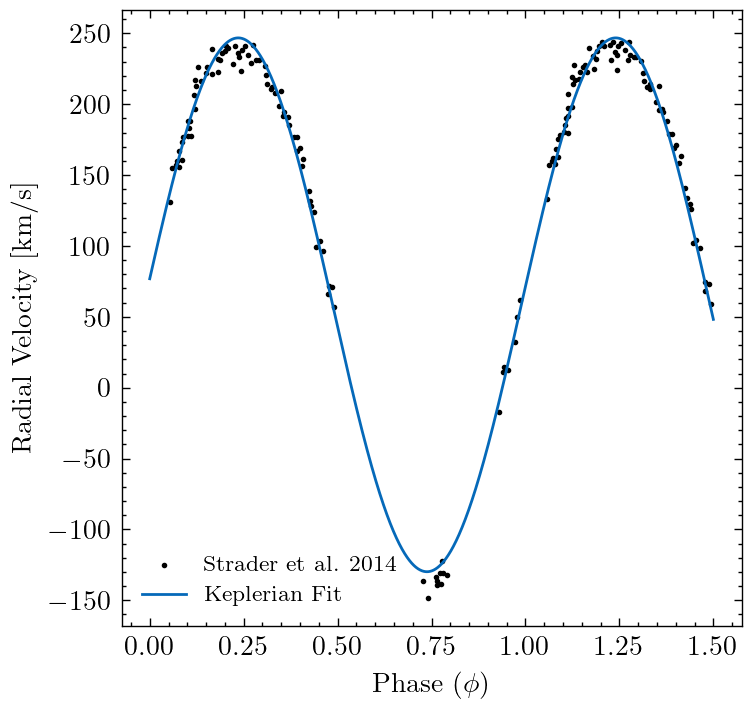
\includegraphics[width = 0.46\textwidth]{figs/radial-velocity.png}}}%
    \qquad
        \subfloat[\centering ]{{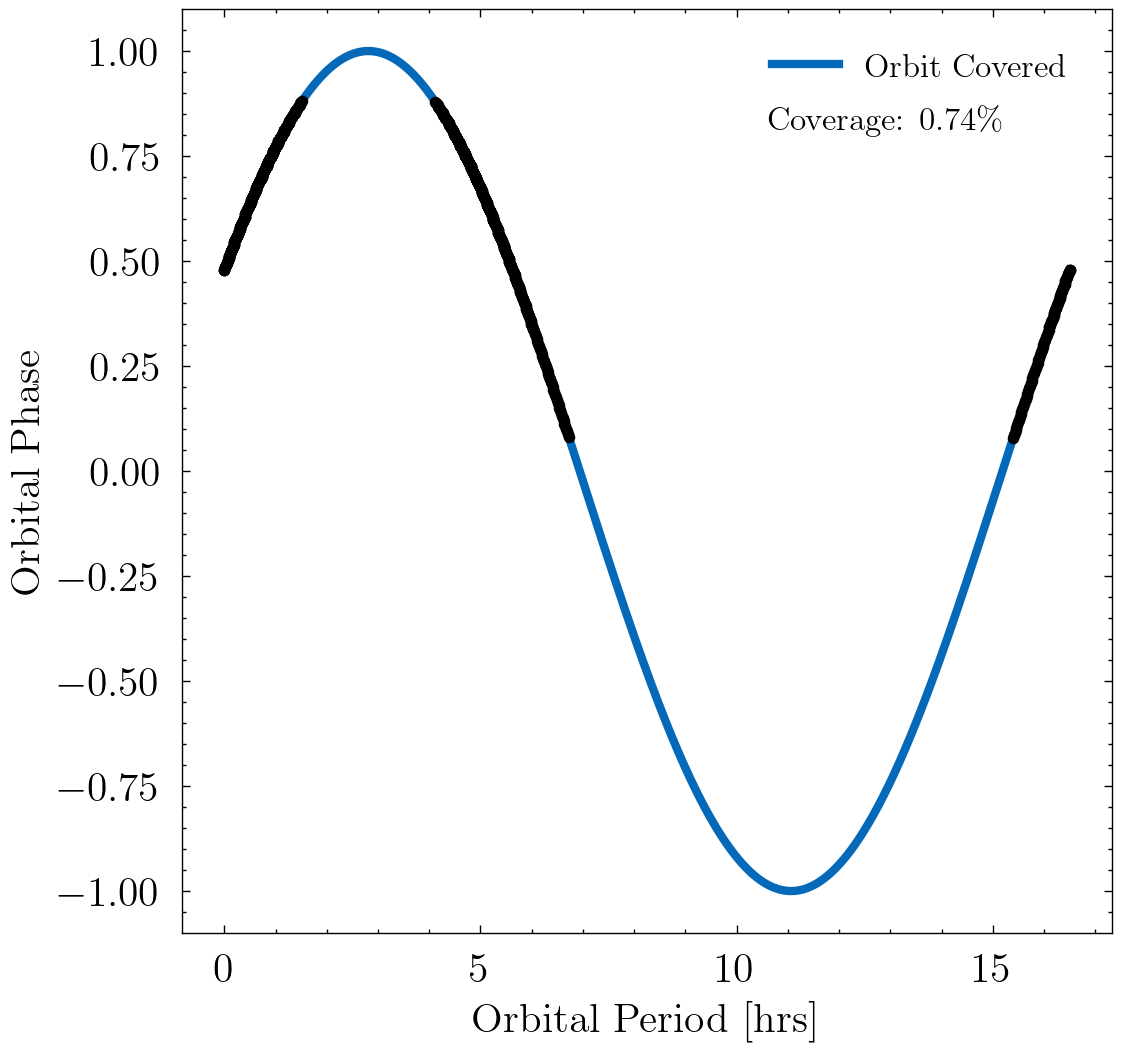
\includegraphics[width=  .46\textwidth]{figs/sine-wave-coverage.png}}}%
    \caption{ }%
    \label{fig: exc5_setup}%
\end{figure}